\documentclass{article}
\usepackage{amsmath, amssymb}  % Paquetes para matemáticas avanzadas
\usepackage{graphicx}  % Paquete requerido para insertar imágenes

\title{Detalles Matemáticos del Código}
\author{}
\date{}

\begin{document}

\maketitle

Consideremos la ecuación presentada en el documento (4):
\begin{equation}
    u''+(1+\epsilon \lambda \omega^2 \cos(\omega \tau))\left(u - \frac{\epsilon^2 u^3}{6}\right) = 0.
\end{equation}

Donde:
\begin{align*}
    \tau &= \omega t, \\
    \omega_0 &= \frac{g}{r_0}, \\
    \epsilon \lambda &= \frac{\delta z}{r_0}, \\
    \omega &= \frac{\omega}{\omega_0}.
\end{align*}

Después de realizar con detalle los pasos para convertir la ecuación diferencial (4) en un sistema de EDOs, vamos a utilizar el **método de Euler mejorado** (también conocido como **método de Heun**) para aproximar las soluciones.

El sistema de EDOs resultante es:
\begin{equation}
    \begin{cases}
        v_1' = v_2,  \\
        v_2' = -(1+\epsilon \lambda \omega^2 \cos(\omega \tau))\left(v_1 - \frac{\epsilon^2 v_1^3}{6}\right).
    \end{cases}
\end{equation}

Donde $v_1 = u$ y $v_2 = u'$. 

## Implementación Numérica

Para resolver este sistema con el **método de Heun**, definimos las siguientes variables iniciales:
\begin{align*}
    \epsilon &= 0.2, \\
    \lambda &= 1.0, \\
    \Omega &= 1.96, \\
    h &\text{ (paso temporal)}, \\
    t_{\text{inicio}} &= 0, \\
    t_{\text{parada}} &= 50.0, \\
    \omega_0 &\text{ (constante de frecuencia angular)}.
\end{align*}

Los valores iniciales son $(0, 0.1)$, es decir, la posición angular es $0$ y la velocidad inicial es $0.1$.

Definimos dos funciones $f$ y $g$ que corresponden a las ecuaciones (1) y (2):
\begin{equation}
    \begin{cases}
        u^* = u_n + h f(t_n, u_n, v_n),  \\
        v^* = v_n + h g(t_n, u_n, v_n).
    \end{cases}
\end{equation}

Estas son las **sucesiones predictoras**, que nos permiten aproximar la posición y la velocidad angular en el tiempo $t_n$. Luego, aplicamos la corrección:
\begin{equation}
    \begin{cases}
        u_{n+1} = u_n + \frac{h}{2} \left( f(t_n, u_n, v_n) + f(t_n + h, u^*, v^*) \right),  \\
        v_{n+1} = v_n + \frac{h}{2} \left( g(t_n, u_n, v_n) + g(t_n + h, u^*, v^*) \right).
    \end{cases}
\end{equation}

En el código, para que esto funcione iterativamente, creamos un ciclo **while** cuya condición de parada es $t_{\text{parada}} = 50.0$. Este ciclo ejecuta las actualizaciones y almacena los datos en un vector para analizar los cambios en la solución.

Ejecutando el codigo podemos ver que la siguiente grafica que muestra como varia la velocidad y posicion angular en el tiempo t

\begin{figure}[h]
    \centering
    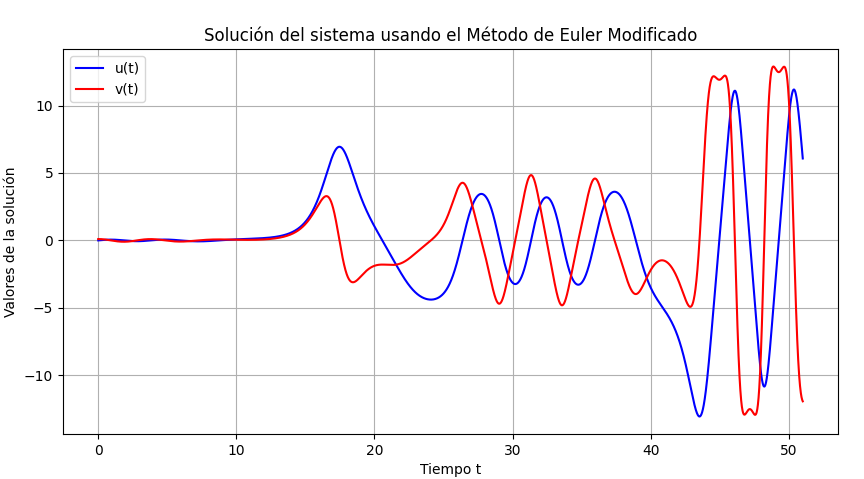
\includegraphics[width=0.9\textwidth]{Captura.PNG}
    \caption{Posicion angular vs velocidad angular}
    \label{fig:etiqueta}
\end{figure}

\end{document}
